
%(BEGIN_QUESTION)
% Copyright 2005, Tony R. Kuphaldt, released under the Creative Commons Attribution License (v 1.0)
% This means you may do almost anything with this work of mine, so long as you give me proper credit

The following ladder logic diagram is for a reversing motor control circuit:

$$\includegraphics[width=15.5cm]{i02496x01.eps}$$

Study this diagram, then explain how motor reversal is accomplished.  Also, identify the function of each "M" contact in the control circuit, especially those normally-closed contacts in series with the motor starter coils.

\vskip 10pt

\filbreak

Now consider the following modification made to the reversing motor control circuit (motor and power contacts not shown here):

$$\includegraphics[width=15.5cm]{i02496x02.eps}$$

What extra functionality do the time-delay relays contribute to this motor control circuit?

\underbar{file i02496}
%(END_QUESTION)





%(BEGIN_ANSWER)

The normally-open and normally-closed "M" contacts provide seal-in and interlock functions, respectively.  The time-delay relays prevent the motor from being {\it immediately} reversed.

%(END_ANSWER)





%(BEGIN_NOTES)

This circuit provides students an opportunity to analyze the workings of a delayed-start, reversing motor control circuit.  Have your students present both their analyses and the methods behind the analyses as you work through this question with them.

\vskip 20pt \vbox{\hrule \hbox{\strut \vrule{} {\bf Virtual Troubleshooting} \vrule} \hrule}

This question is a good candidate for a ``Virtual Troubleshooting'' exercise.  Presenting the diagram to students, you first imagine in your own mind a particular fault in the system.  Then, you present one or more symptoms of that fault (something noticeable by an operator or other user of the system).  Students then propose various diagnostic tests to perform on this system to identify the nature and location of the fault, as though they were technicians trying to troubleshoot the problem.  Your job is to tell them what the result(s) would be for each of the proposed diagnostic tests, documenting those results where all the students can see.

During and after the exercise, it is good to ask students follow-up questions such as:

\begin{itemize}
\item{} What does the result of the last diagnostic test tell you about the fault?
\item{} Suppose the results of the last diagnostic test were different.  What then would that result tell you about the fault?
\item{} Is the last diagnostic test the best one we could do?
\item{} What would be the ideal order of tests, to diagnose the problem in as few steps as possible?
\end{itemize}

%INDEX% Electronics review: time-delay relay

%(END_NOTES)


